%%%%%%%%%%%%%%%%%%%%%%%%%%%%%%%%%%%%%%%%%%%%%%%%%%%%%%%%%%%%%%%%%%%%%%%%%%%%%%%%
%2345678901234567890123456789012345678901234567890123456789012345678901234567890
%        1         2         3         4         5         6         7         8

\documentclass[letterpaper, 10 pt, conference]{ieeeconf}  % Comment this line out if you need a4paper

%\documentclass[a4paper, 10pt, conference]{ieeeconf}      % Use this line for a4 paper

\IEEEoverridecommandlockouts                              % This command is only needed if
                                                          % you want to use the \thanks command

\overrideIEEEmargins                                      % Needed to meet printer requirements.

%In case you encounter the following error:
%Error 1010 The PDF file may be corrupt (unable to open PDF file) OR
%Error 1000 An error occurred while parsing a contents stream. Unable to analyze the PDF file.
%This is a known problem with pdfLaTeX conversion filter. The file cannot be opened with acrobat reader
%Please use one of the alternatives below to circumvent this error by uncommenting one or the other
%\pdfobjcompresslevel=0
%\pdfminorversion=4

% See the \addtolength command later in the file to balance the column lengths
% on the last page of the document

% The following packages can be found on http:\\www.ctan.org
\usepackage{graphics} % for pdf, bitmapped graphics files
\usepackage{epsfig} % for postscript graphics files
\usepackage{mathptmx} % assumes new font selection scheme installed
%\usepackage{times} % assumes new font selection scheme installed
\usepackage{amsmath} % assumes amsmath package installed
\usepackage{amssymb}  % assumes amsmath package installed
%\usepackage{algorithmicx}
%\usepackage[Algorithm,ruled]{algorithm}
%\usepackage{algpseudocode}
\usepackage{tabularx}
\usepackage{multirow}
\usepackage{color}
\usepackage{url}
%\usepackage{balance}
\usepackage{subcaption}
\usepackage{breqn}
\usepackage{algorithm2e}
\usepackage{dblfloatfix} 
\usepackage[export]{adjustbox}
\usepackage{tabulary,booktabs}
%\usepackage{verbatim}
%\usepackage{flushend}
\usepackage{float}

\newcommand{\junk}[1]{}
\newcommand{\abs}[1]{\left| #1 \right|} %| |
\newcommand{\comment}[1]{\textcolor{red}{#1}}

\title{\LARGE \bf
Autonomous Pick and Place Grasping Task, using RGB-D Camera and Bumper Sensing
}
\author{Mohamed Shire, Hou Nam Chiang, Renjie Zhou}

\date{01 January 2021} %it will not be displayed

\begin{document}

\maketitle
\thispagestyle{empty}
\pagestyle{empty}

\section{INTRODUCTION}\label{Sec:intro}
% Pick and place has been an age-old problem in robotics, where a robot grasps, places and then ungrasps an object. Being able to precisely transport an object in space is an essential skill that humans take for granted. Solving the pick and place problem makes it such that repetitive actions in a factory line can be automated, freeing up labour for other more complex tasks. Pick and place robots have been proven to drastically increase the efficiency of factories, greatly increasing the speed and consistency of production lines by taking part in the assembly and quality assurance of products. %insert reference for this section
% This report will be looking at implementing a pick and place robot with the aid of an RGB camera and bumper sensors. 

Robotic research has consistently been seeking for improved efficiency and productivity at a lower cost. Pick and place has been an age-old problem in robotics, where a robot grasps, places and then ungrasps an object. Automating the pick and place problem with accuracy and efficiency frees up manual labour for other more complex tasks, increasing the productivity \cite{ifr2017}. 

However, the environment in real life is always complex. Apart from the object of interest, many other objects are usually on scene, resulting in potential collision with the robot when performing the pick-and-place task. Hence visual and touch sensors are required for object detection. However, in places like factory with big open space, where high-precision and high-accuracy exteroceptive sensors may not be easily available or even feasible. 

Hence, we propose to use only two types of sensors, namely RGB-D camera and bumper sensors, to learn about the environment and perform the task such as pick and place in a constrained environment with obstructions in scene. We propose to store the information of the objects on the scene using point cloud and handle object extraction using Point Cloud Library (PCL). Then we proceed to use \texttt{ROS} to communicate cylinder coordinates and bumper sensor data information for pick-and-place tasks.

%motivation
%problem definition
%who benefits from solution
%solution outline
%why has the problem not been solved
%need to have multiple paragraphs
\section{PROBLEM SETUP}
The problem we are facing here is to use the information from RGB-D camera and bumper sensors to perform the object detection and solve pick-and-place via grasping under constraints of potential obstructions that need to be cleared from the designated surface. 

There are two parts of this problem. First, there needs to be a way to detect and locate the initial position and orientation of the target in the 3D scene. Second, the robot needs to pick up the target and place it onto the designated surface under the constraints, such as the designated surface being occupied by other objects. Hence, the robot needs to know the latest pose of the targeted object so that it knows where to grasps the target. The robot also needs to know whether the designated surface is free, and if not, where to move the obstructions to. We will be further discussing the existing work to handle the above-mentioned problems and their limitations.
\section{RELATED WORK}
As the problem can be subdivided into two parts, we have looked into the two sections: object detection and segmentation and detection of hindering objects in the environments. 
\subsection{Object detection and segmentation}
%can discuss how other work has used image recognition or point cloud for such task and the limitations
%What are point clouds?
There exists various ways of detecting objects in robotic research. Many work with pick-and-place and sorting as the final goal implements image processing, segmentation and 
classification to detect and categorise the object. Kumar et al. has used feature extraction, ``Canny Method" based edge detection followed by classification using the Artificial Neural Network (ANN)\cite{kumar2014}. Vijayalaxmi et al. has used grey-level image segmentation and pre-defined positions on the conveyor belt for object detection and identification\cite{VIJAYALAXMI2013}. However, these methods are mainly for object detection and classification in 2D, and not really provide depth information of the object. Moreover, the classification is not part of the task in the problem we want to study. We then looked into the work by Tsarouchi et al., who have combined 2D vision system with data from computer-aided design (CAD) files for generation of 3D coordinates\cite{Tsarouchi2016}. However, this requires storage, mapping and maintenance of both the CAD data and vision data. Also, not all objects can be generated in CAD. 
Börcs et al. has discussed the effective object detection method using point cloud formed by using LiDAR, followed by a classification using Convolutional Neural Network (CNN) to effectively segment, extract and identify the objects\cite{Borcs2017}. 

% A point cloud is a set of 3D points that correspond to the X, Y and Z planes. These are typically gathered from: 1) Image methods, 2) Light Detection and Ranging, 3) Red Green Blue Depth (RGBD) cameras and 4) Synthetic Aperture radar (SAR) systems [1].  Depending on the type of scanning method used, extra dimensions of data can be appended to the standard point cloud, an example of this would be the RGB data of a point. The different point cloud acquisition methods also have different use cases, while lidar systems can operate even from airborne aircrafts, RGB-D cameras are restricted in range and are typically used to map indoor environments [1]. With scanning technologies becoming more accessible in recent years, the point cloud library (PCL) developed in 2011 [2] has become an essential means of processing point cloud datasets. 

% %What is segmentation?
% A fundamental step of processing point clouds is segmentation. Like image segmentation, point cloud segmentation is the clustering and labelling of point clouds regions into different categories.  The segmentation of both images and point clouds have multiple applications, examples include: the tracking, locating and classification of objects [3]. 

% %Application of points clouds.

% %The data acquired from RGB-D cameras are typically used for plane segmentation methods [1]. Indoor objects such as walls, ceilings, tables are all planar in nature. The extraction of the plane of these objects can prove to provide a comprehensive representation of the point clouds [4]. Plane segmentation is a complex task generally used for indoor reconstruction and mapping [4].

% %Point cloud segmentation techniques
% There are several point cloud segmentation techniques. These can be categorized into edge-based methods, region-based methods, model-based methods and graph-based methods [2]. Each of the groups of methods have pros and cons associated with them, we will briefly look at the differences in the approaches of these techniques.

% Edge based methods look to detect and isolate edges as they are seen as the boundary between clusters of point clouds. The idea is to find the areas of point clouds where there is a rapid change of intensity [2]. An example of an edge based algorithm can be seen as presented by Wani and Arabnia (2003). As these groups of algorithms are only concerned with a subset of the point cloud data (edge regions), they prove to be computationally efficient [wani]. While edge-based methods can provide quick results, the accuracy is questionable as they are very sensitive to noise and outliers [2]. 

% Region based methods assume that nearby points share similar properties [4].The algorithms start around an initial set of seed points, and then expands to neighbouring points that share characteristics [techn]. Initially, similar regions were identified based on proximity, and planarity of regions [techn]. Soon, variations of region based algorithms as seen in [Vosselman] proposed using colour as another similarity criteria. These methods find it difficult to find a solution between under and over segmentation [3]. This group of methods also struggles to distinguish between regions with seamless and smooth transitions between them. For these cases finding criteria for region termination becomes difficult [4]. Region based methods are better at handling outliers than edge based methods as they consider global point cloud data rather than a subset, however they are particularly sensitive to the initial seed locations[techn].

% Model based methods use simple geometric shapes (plane, cylinder, cone) for grouping clusters of point clouds [3]. Points with similar mathematical representations are grouped under the same region [3]. An example of a model-based method is the famous Random Sample and Consensus (RANSAC) method. This model is used to detect geometric features such as straight lines and circles [3]. The RANSAC method is current state of the art, it is an iterative method that works by identifying the outliers of a dataset and fitting a model based on the remaining data[core]. While the RANSAC method is robust in that it is not affected by outliers and noise to the scale of other methods, an issue is that the planes detected by RANSAC may not be of the same surface [4]. As this method focuses on fitting geometrically simple shapes, it also struggles when faced with more complex shapes[core2]. 

% Graphical methods view the cluster of point clouds as a graph. With each vertex being a point and the edges connecting some pairs of neighbouring points [2]. These group of methods are typically very efficient and has seen usage in robotic applications [2].

%Pick and place under constraints - finding limitations of these other 
\subsection{Detection of hindering objects in the environment}
The ability to detect and avoid obstacles is one of the most basic functions an autonomous robot should have. The use of LIDAR, sonar and cameras as sensors is common in the field of object detection. Romdhane et al have explored obstacle detection for collision avoidance through the use of monocular and stereo camera approaches \cite{BenRomdhane2011}. However, monocular based methods are heavily dependant on a prior of an approximated location of the object for obstacle detection \cite{BenRomdhane2011}, which may not be always available. 

In recent years, RBGD cameras have been widely explored as an alternative as they overcome the planar limitations of the previously mentioned sensors, providing real-time fulcrum based depth readings \cite{Peasley2013}. Peasley et al have suggested mounting an RBGD camera on the front of the mobile robot. The 3D point cloud is then transformed to a birds-eye view to create a map of obstacles in the current field of view of the objects\cite{Peasley2013}. This approach, however, is constrained to an indoor environment as a ground-plane constraint was applied. This is where it is assumed the robot will be traversing a flat ground plane, and anything above the identified ground plane can be a potential obstacle \cite{Peasley2013}. Since the robot is traversing the ground, any obstacles detected with a height above 0.5m were filtered out as the object would not be at risk of colliding with surfaces of that height. By obtaining a planar obstacle map, obstacle avoidance algorithms can then be employed. 

Similarly,  Singh et al described their obstacle detection process as first segmenting point clouds into ground and non-ground planes. Then through the use of feature extraction methods, obstacles in the cameras view can be identified \cite{Singh2017}. These methods are useful and effective when the initial locations of the hindering objects are unknown or changing.

%While this is an effective method for obstacle detection, this approach is limited in that the 3D problem has been transformed to a planar problem. This approach cannot be applied to a pick and place robot, when an object of interest could be placed on-top of an obstacle.




% can talk about how other people have detected the hindering object and the limitations



\section{METHODOLOGY}\label{Sec:proposal===}
This paper proposed using visual and touch sensors only to perform the automatic pick and place grasping task in a constrained environment with given surfaces and initial location of the hindering object. The visual sensor used in the study is a RGB-D camera and the touch sensors used are bumpers. Both are for object detection purpose. We proposed to extract a three-dimensional point cloud of the cylinder using RGB-D camera. We decided to use the PCL mentioned earlier for point cloud processing and object segmentation and extraction. We applied various filters such as voxel-grid, which uses clustering to down sample the size of the point clouds, and pass through filters, which filter out points irrelevant to the objects we are interested, to reduce the number of points in the cloud. As the  extraction of the location and height of the cylinder needs to go through every point in the cloud, decreasing the number of points lowers the computational complexity of cylinder extraction. 

We then use model based extraction methods to extract and remove the plan surface to facilitate extraction of cylinder. A mathematical approach is taken to calculate the normal of the remaining points to find the points with similar normal as the cylinder to extract the cylinder. Following that, the extracted normal is used to extract the cylinder using model based extraction with mathematical parameters of an infinite cylinder. The height of the cylinder is determined using the coordinates of the highest and the lowest point in the point cloud. 

After the cylinder is detected, we keep track of the latest cylinder pose. We also detect and track whether the surface that cylinder is supposed to be moved to is free from any other object by using bumper sensors. Each surface has a bumper sensor located at the centre that notifies whether the surface is occupied. If occupied, a pick-and-place is performed to move the object to some other unoccupied table before placing the cylinder. The robot only receives which surface to put the cylinder as input information from the users, and perform the rest of the tasks automatically. Hence, Our proposed algorithm needs to handle the detection of any object on the designated table, clearing of the object and pick-and-place of cylinder to transport it to the designated surface. The details of the experimental setup and the simulations are introduced in section \ref{sec:exp}. 
\section{EXPERIMENTS}\label{sec:exp}
\begin{figure}[h]
    \centering
    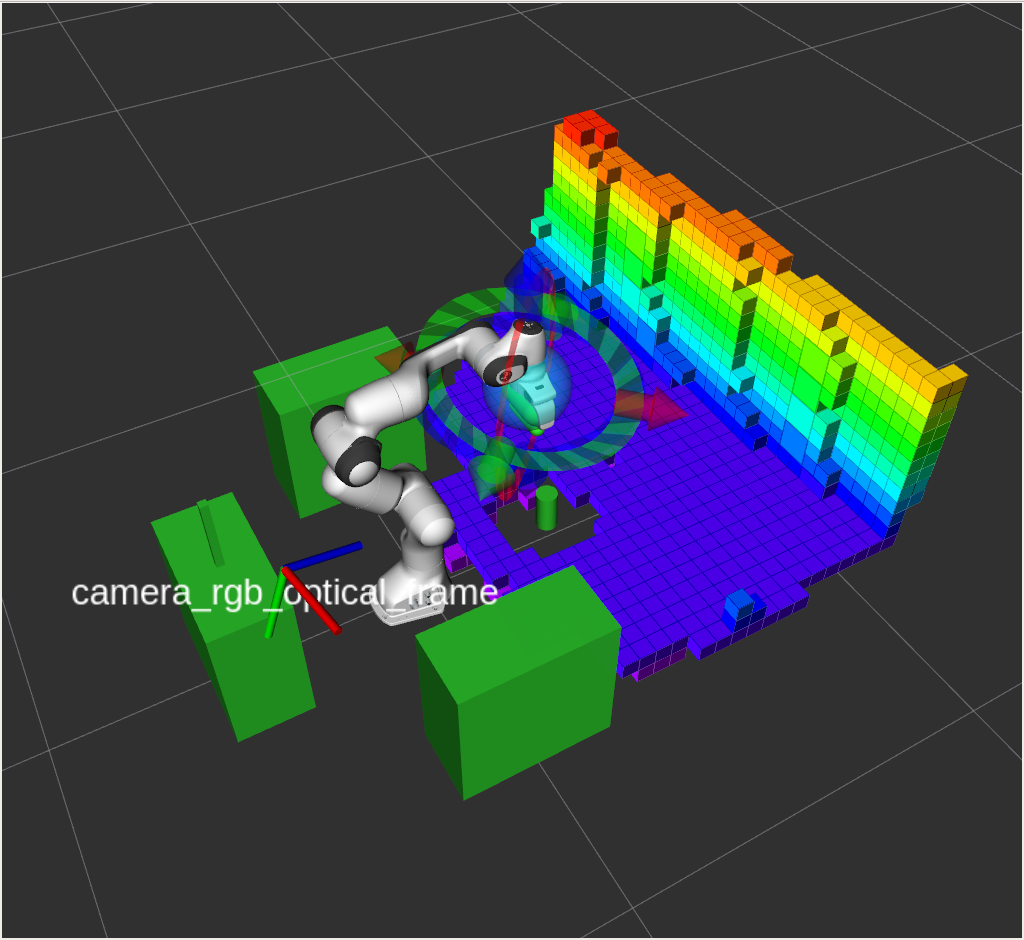
\includegraphics[width=5cm]{figures/exp2.png}
    \caption{Experimental setup}
    \label{fig:exp_setup}
\end{figure}
Due to the COVID-19 situation, we couldn't have the access to actual equipment and therefore proceed with simulations to experiment our algorithms for automatic pick-and-place grasping. 

Here we are using PANDA Robotic Arm with 7 degrees of freedom. We set the environment to contain one surface of wall and plane and three cubes of dimension 0.2$\times$0.4$\times$0.4 on the scene as shown in figure \ref{fig:exp_setup}, namely ``table1", ``table2" and ``table3".At the centre of each table, there is a bumper sensor to detect whether the table is occupied, namely ``bumper1", ``bumper2" and ``bumper3". A RGB-D camera is installed behind the robot, facing the wall, as shown in the \ref{fig:exp_setup}, for detecting objects on scene and forming point cloud. At the beginning, there is an object of dimension 0.02$\times$0.02$\times$0.2 on table2, which results in the bumper2 informing the robot that table2 is occupied, whereas the the other two bumper sensors inform the robot of the unoccupied surface. 

We will be having access to two information sources: the latest cylinder pose and the three bumper sensors' data. We used \texttt{PCL} and \texttt{ROS} in our simulation experiments. The cylinder pose is updated and published to the \textt{ROS} topic \texttt{/cylinder\_pose}, and the data from the bumper sensors is published to \textt{ROS} topic \texttt{/bumper1}, \texttt{/bumper2} and \texttt{/bumper3}, with \texttt{/bumper2} publishing boolean messages of ``true" and others publish ``false" to indicate only table2 is occupied at the beginning. 

Our experiments include testing the increase in extraction speed by applying various filters to the point cloud, the grasp of object, the process of pick-and-place to transfer the cylinder from the ground onto a free table, and the similar process of transferring the cylinder to an occupied table, which involves the removal of the object from the table. The results and discussions are detailed below.

\subsection{Increase in speed of cylinder extraction}
We have experimented various filters to speed up the cylinder extraction and test the time reduced. Below is the table to show the impact of the filtering on the time taken to extract the cylinder.
\begin{table}[h]
    \centering
    \begin{tabular}{|m{3cm}|m{1cm}|m{2cm}|}
        \hline
        Action & Number of points & Time of cylinder extraction (microseconds)  \\
         \hline
         RGB-D camera scan & 307200 & NA\\
         \hline
         Pass through filter to identify region of interest with range applied on z axis & 83484 & 4278 \\
         \hline
         Basic pass through filter + voxel grid filter to down sample the cloud & 5687 & 490\\
         \hline
         Basic pass through filter + pass through filter (fast filter) identifying the region of cylinder & 43122 & 2995\\
         \hline
         Basic pass through + voxel grid filter + fast filter & 2769 & 384\\
         \hline
    \end{tabular}
    \caption{Impact of applying different filters on speed of cylinder extraction}
    \label{tab:filters}
\end{table}

As shown in table \ref{tab:filters}, the voxel grid filter alone is more effective than fast filter alone in extraction speed boost. However, the combined effect of voxel grid and fast filter is the best.

\subsection{Grasp of cylinder from ground to surface}
\begin{figure}[h]
    \centering
    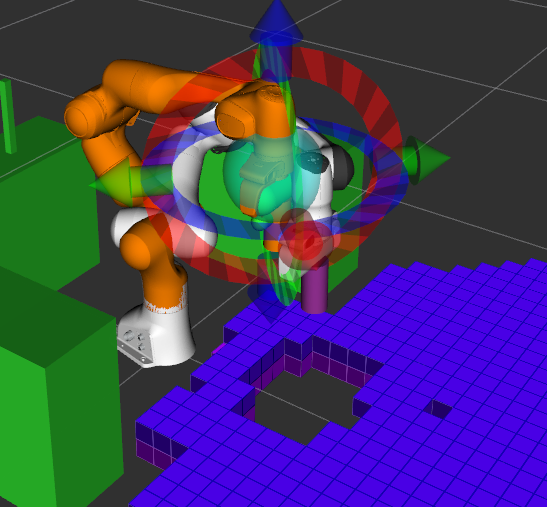
\includegraphics[width=4cm]{figures/grasp1.png}
    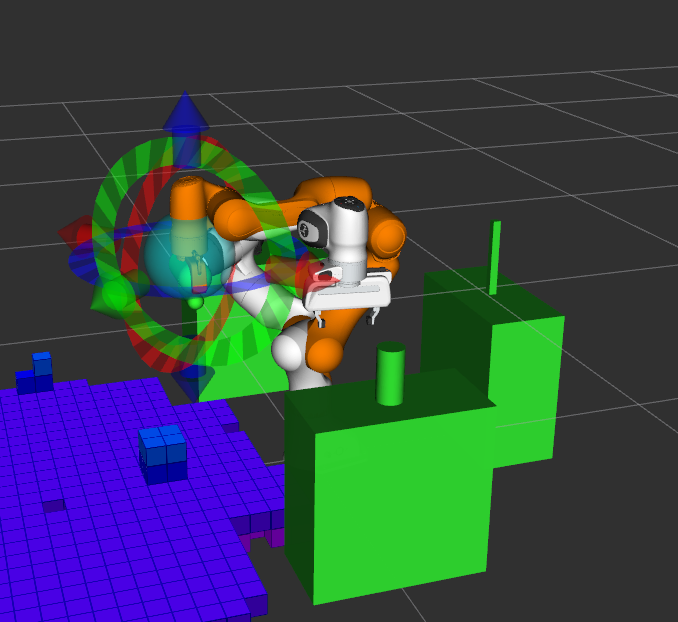
\includegraphics[width=4cm]{figures/grasp2.png}
    \caption{Picking up the cylinder and placing onto table1}
    \label{fig:grasp}
\end{figure}
As shown in figure \ref{fig:grasp}, upon receiving ``1" as the input, the robot successfully automatically locates the position of the cylinder, picks up the cylinder and place it onto table1.

\subsection{Automatic pick and place of cylinder in constrained environment}
\begin{figure}[h]
    \centering
    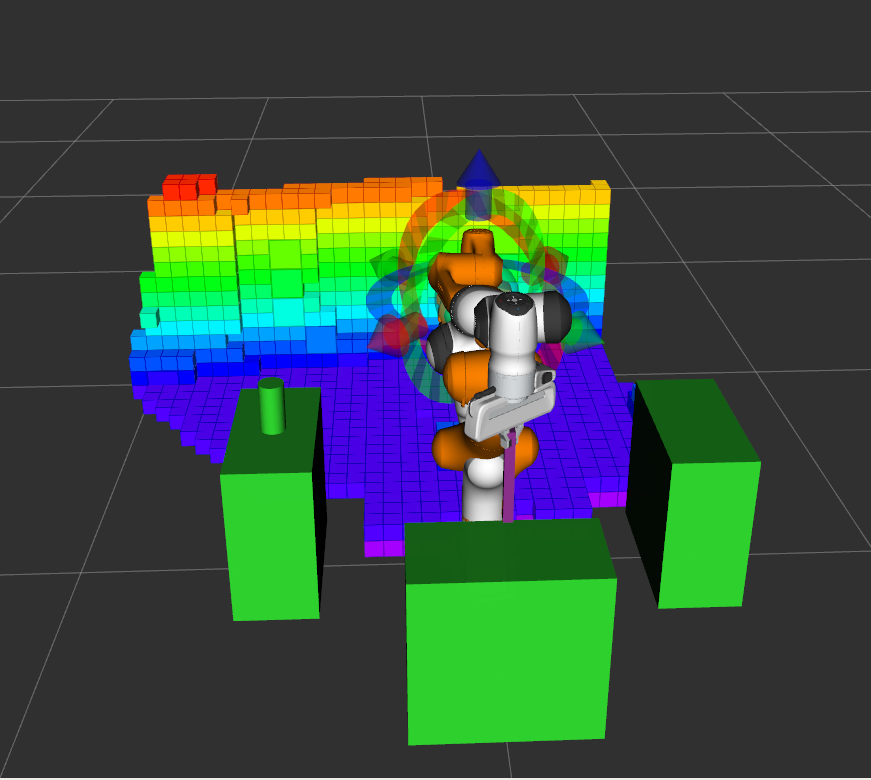
\includegraphics[width=4cm, height=4cm]{figures/2_pickStick.png}
    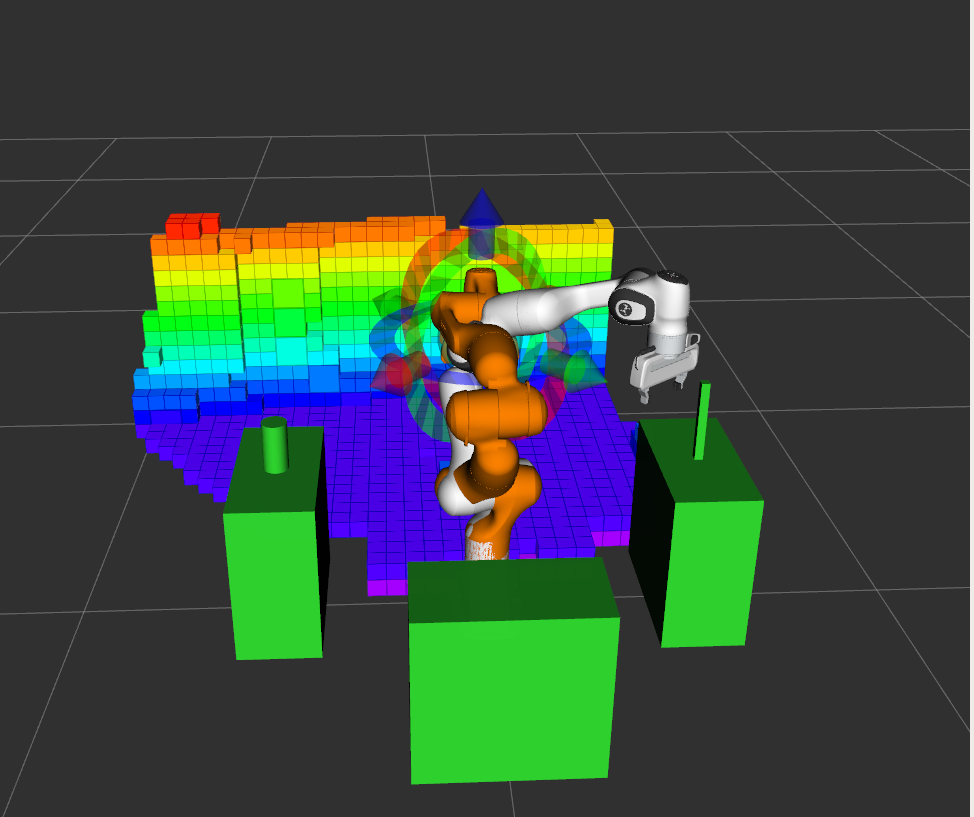
\includegraphics[width=4cm, height=4cm]{figures/2_placeStick.png}\\
    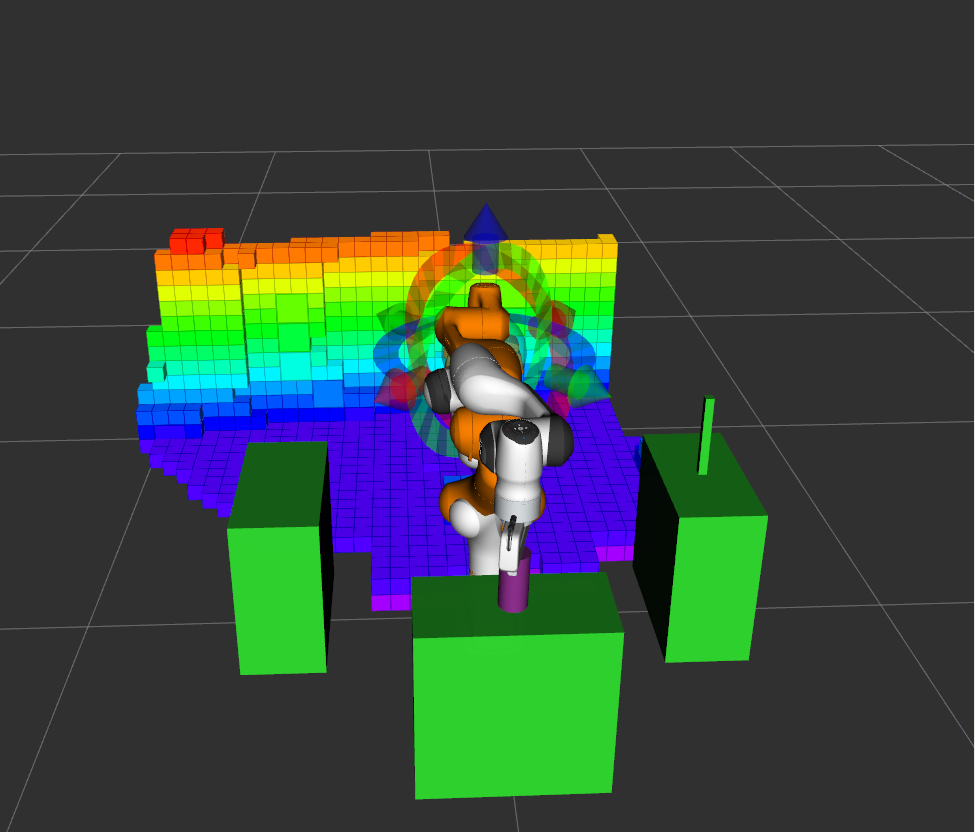
\includegraphics[width=4cm, height=4cm]{figures/2_pickCylinder.png}
    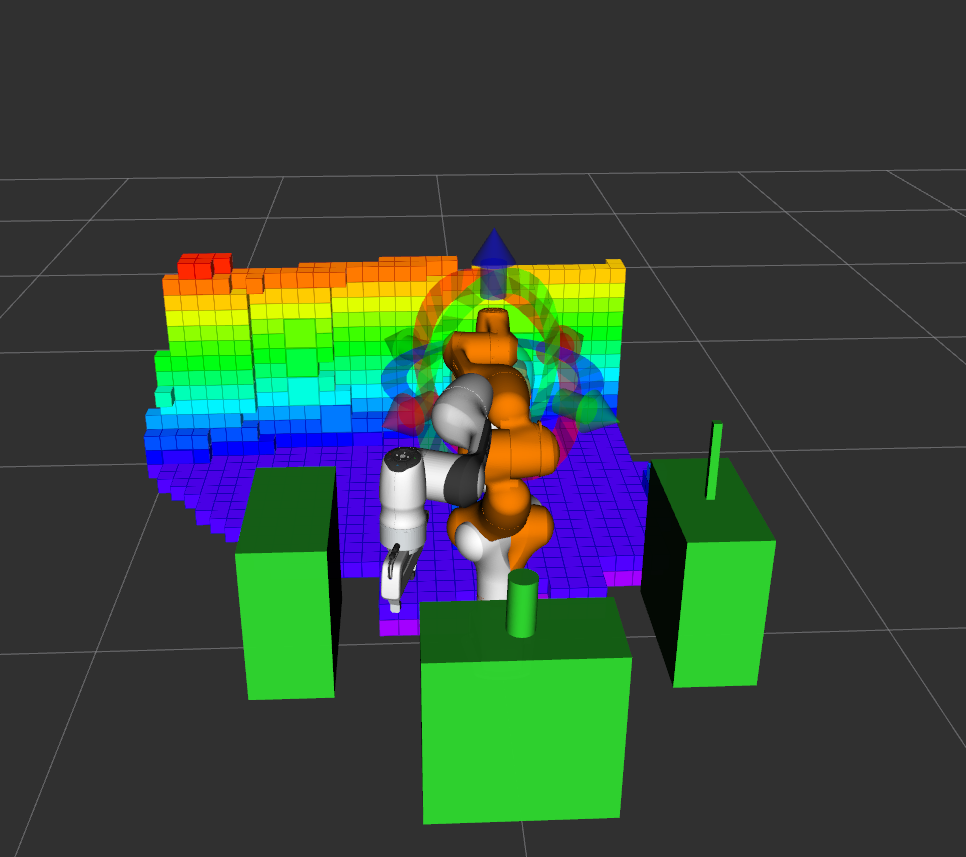
\includegraphics[width=4cm, height=4cm]{figures/2_placeCylinder.png}
    \caption{Picking up the cylinder and placing onto table1}
    \label{fig:2_pickPlace}
\end{figure}
As shown in the figure \ref{fig:2_pickPlace}, upon receiving instructions, the robot will automatically detect whether the designated table is occupied, and, if so, moves the occupant to another free table before placing the cylinder there. In this case, when the user input is ``2", the robot detects that there is an object on the table 2, and moves the object from table 2 to table 3 upon detecting that table 3 is empty, before moving the cylinder from table 1 to table 2. \\

From the simulated experiments, we can see that the algorithm we developed using RGB-D camera and bumper sensors can successfully detect the presence of objects on the surfaces and automate the process of pick-and-place of the target under the constraints of having obstructions on the surfaces. \\

However, the experiments conducted in the simulation are largely simplified. The context of the constraints in the environment can be much more complicated. For example, most objects may not be placed right at the center on the surface in real life, and therefore may not be detected if there is only one bumper sensor at the center of the table. It could also be that there are many obstructions on the scene and the RGB-D camera cannot detect the target of interest, therefore cannot generate the 3D point cloud of the object. These limitations need further considerations when conducting experiments in real life.
\section{CONCLUSION AND FUTURE WORK}\label{Sec:concl}
% I will keep this document updated when new techniques are needed.  Google is always there for you to find the right way to write in $\LaTeX$, although you can also read any $\LaTeX$ Cheat Sheet, e.g.\\ \url{https://www.nyu.edu/projects/beber/files/Chang_LaTeX_sheet.pdf}
\subsection{Conclusion}
In conclusion, we have developed the algorithms to successfully solve the automation of the pick-and-place problem of a target of interest in a simplified constrained environment. This work only requires the 3D point cloud generated from the RGB-D camera and the bumper sensors located on the surfaces. However, as the experimental setup is much simplified, possibly more sensors (e.g. one more RGB-D camera to capture the target of interest from different angles, or more bumper sensors to cover the entire surface) may be needed to successfully complete the autonomous pick and place in real life scenarios.  


\subsection{Future Work}
As described, more work can be done to improve the algorithm to work better in a more complex real-life scenario, such as incorporating more than one RGB-D camera or bumper sensor data. Also, we can look into object identification by implementing classification algorithms such as CNN models for image recognition for further functions, such as picking up the required objects input by users and put them to the designated tables.   


\bibliographystyle{IEEEtran}
\bibliography{references}
\end{document}